% -----------------------------------------------------------------
% Experimental Evaluation section (insert after Implementation)
% -----------------------------------------------------------------
\section{Experimental Evaluation}  % -- Section IV --

% ===================== 4.A Evaluation Metrics ====================
\subsection{Evaluation Metrics}  % -- 4.A --
% -- List metrics used and give formulas --
To rigorously assess model performance we employed standard metrics:
accuracy, precision, recall, and the Area Under the Receiver Operating
Characteristic Curve (ROC–AUC). Accuracy is defined as the proportion
of correctly identified instances:
\begin{equation}
\text{Accuracy} = \frac{TP + TN}{TP + TN + FP + FN},
\end{equation}
where $TP$, $TN$, $FP$, and $FN$ denote true positives, true negatives,
false positives, and false negatives, respectively.
Precision and recall are given by
\begin{equation}
\text{Precision} = \frac{TP}{TP + FP},
\qquad
\text{Recall}   = \frac{TP}{TP + FN}.
\end{equation}
ROC–AUC provides an aggregate view over all possible classification
thresholds and is particularly useful when operating conditions vary.

% ===================== 4.B Dataset & Setup =======================
\subsection{Dataset and Experimental Setup}  % -- 4.B --
% -- Corpus description and split protocol -----------------------------------
All experiments used the labelled human- and AI-authored texts provided by
Kaggle’s \emph{Detect AI-Generated Text} corpus.  After deduplication, the dataset was stratified and partitioned in a
70 : 15 : 15 ratio for training, validation, and in-domain test sets,
respectively. {The split was fixed with a global random seed for
reproducibility.}

% ===================== 4.C Baseline Evaluation ===================
\subsection{Baseline Model Evaluation}  % -- 4.C --
% -- Naive Bayes, Logistic, SGD results overview --
Baseline models—Multinomial Naïve Bayes, Logistic Regression, and
Stochastic Gradient Descent (SGD)—were trained on TF–IDF features.
They achieved moderate accuracy but struggled with sophisticated
GPT-4-level content, highlighting limitations of shallow representations.

% ===================== 4.D Advanced Evaluation ===================
\subsection{Advanced Model Evaluation}  % -- 4.D --
% -- CatBoost and BERT performance overview --
Advanced approaches (CatBoost, LightGBM, and BERT) were
then evaluated. CatBoost excelled on sparse, high-dimensional data,
while BERT captured deeper semantics and context. Both required careful
hyper-parameter tuning; BERT additionally demanded significant
computational resources.

% ===================== 4.E Hyper-parameter Tuning ===============
\subsection{Fine-Tuning and Hyperparameter Optimization}  % -- 4.E --
% -- Grid search over vectorizer + model params --
Grid search was employed to optimise vectoriser settings
(\emph{n}-gram range, max features) and model hyperparameters
(regularisation strength, class weights, learning rate, depth). The
resulting configurations yielded noticeable gains in accuracy and
generalisation.

% ===================== 4.F Independent Test Evaluation ==========
\subsection{Independent Test Set Evaluation}  % -- 4.F --
% -- Domain-shift performance drop discussion --
When models were applied to the external test set, all experienced a
decline in accuracy as shown in picture \cref{fig:model_against_independent}, underscoring domain-shift and data distribution
challenges. This performance drop indicates that robust, adaptive
detectors are necessary for real-world deployment.

\begin{figure}[tb]
  \centering
  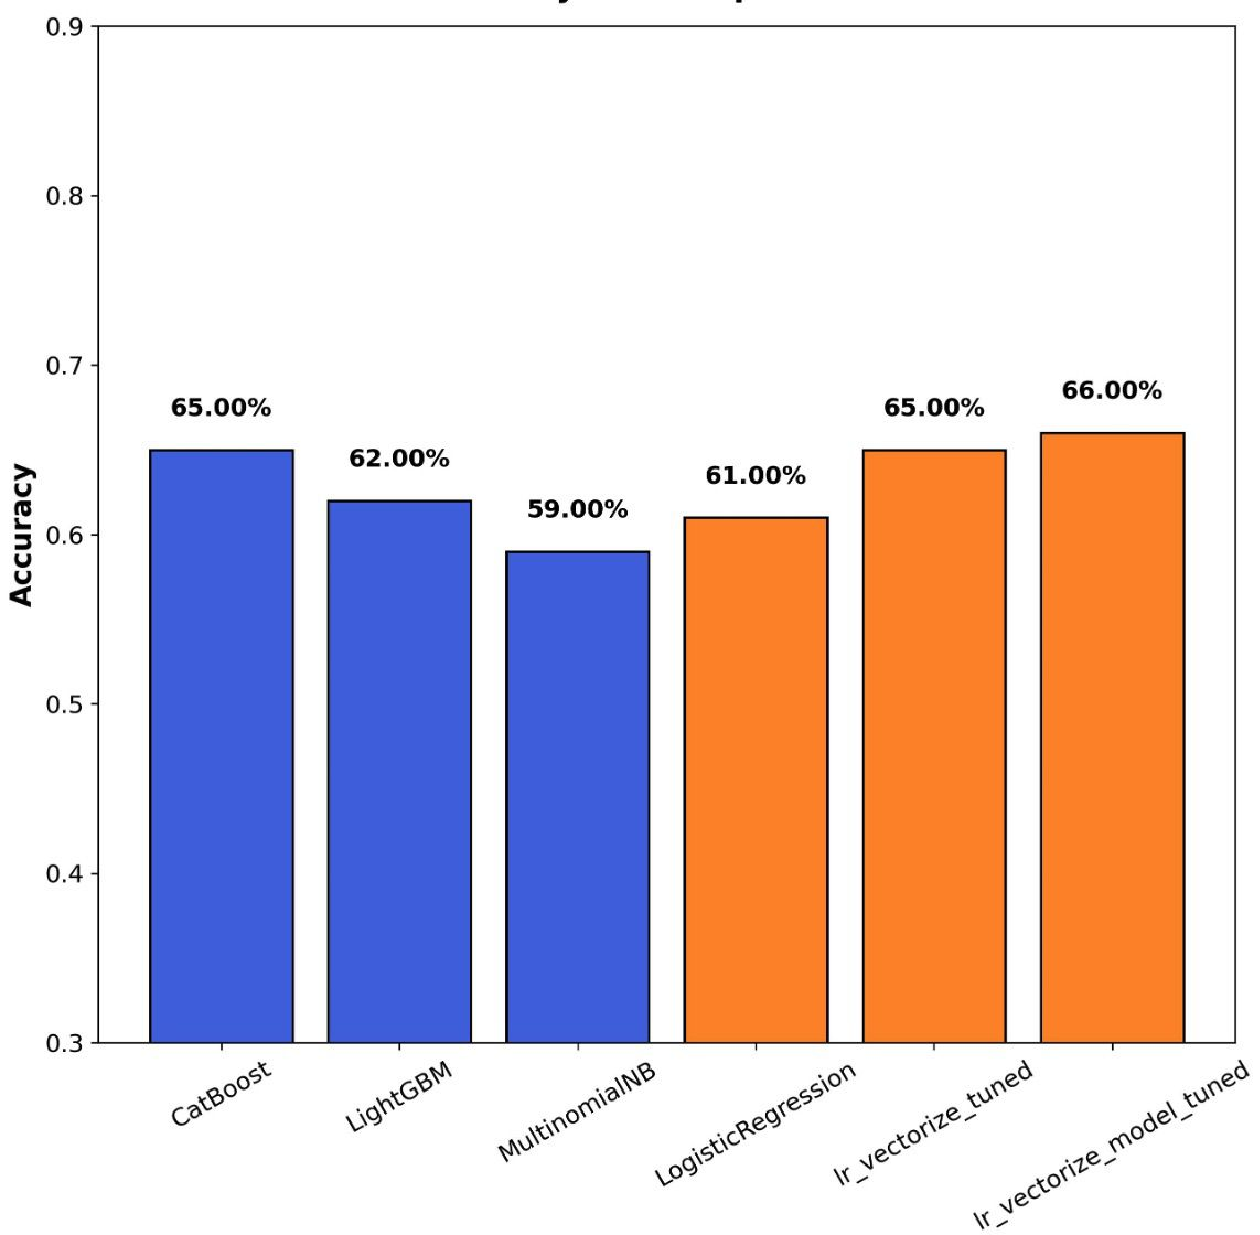
\includegraphics[width=\linewidth]{model_against_independent.pdf}
  \vspace{-20pt}
  \caption{Model accuracy against independent dataset}
  \label{fig:model_against_independent}
\end{figure} 

